\documentclass{report}

\usepackage{ugentstyle}
\usepackage{amsmath}

\begin{document}
	\maketitle{Gevorderde algoritmen}
	\tableofcontents
	\part{Theorie}
	\chapter{Inleiding}
	Het vak gevorderde algoritmen behandelt vier luiken:
	\begin{enumerate}
		\item \textbf{Gegevensstructuren}. Dit onderdeel behandelt meer efficiënte zoekbomen zoals Rood-zwarte bomen, Splay trees, B-trees en meerdimensionale gegevensstructuren zoals Quadtrees en k-d trees. Er wordt ook bekeken hoe zeer grote datastructuren (die niet vollledig in het geheugen passen) behandelt worden.
		
		\item \textbf{Grafen}. Een uitbreiding op de grafentheorie. Onderwerpen zoals stroomnetwerken, \todo{aanvullen wanneer stof gezien is}
		
		\item \textbf{Strings}. Dit hoofdstuk gaat dieper in op stringfuncties. Een aantal onderwerpen zijn efficiënte zoekmethoden, de theorie achter reguliere expressies en hun grammatica en het samenvatten van teksten.
		
		\item \textbf{Complexe problemen}. Dit onderdeel behandelt de NP-problemen. Wat zijn ze? Hoe kunnen we NP-problemen transformeren naar een eenvoudiger probleem? Hoe kan men benaderde oplossingen gebruiken?  
	\end{enumerate}
	\chapter{Efficiënte zoekbomen}
	\section{Herhaling binaire zoekbomen}
	Een binaire boom is een belangrijke boomstructuur waarin drie operaties belangrijk zijn: \textit{zoeken, toevoegen en verwijderen}. Deze drie operaties worden kort herhaald op figuur \ref{fig:bin_boom_1}
	
	\begin{figure}[h]
		\centering
		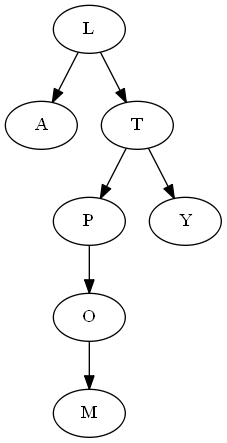
\includegraphics[width=5cm,height=5cm,keepaspectratio]{bin_boom_1}
		\caption{Een binaire zoekboom.}
		\label{fig:bin_boom_1}
	\end{figure}

	\begin{itemize}
		\item \textbf{Zoeken} naar een knoop komt overeen met binair zoeken. Stel dat we knoop P zoeken dan weten we dat dit groter is dan L dus gaan we naar rechts, en kleiner is dan T dus gaan we naar links.
		
		\item \textbf{Toevoegen} van een knoop komt overeen met zoeken naar die knoop, en dan de knoop op die positie toe te voegen. Stel dat we een knoop Q willen toevoegen, dan zal het binair zoeken leiden dat deze knoop in het rechterkind van P moet komen, zoals te zien op figuur \ref{fig:bin_boom_2}
		
	\begin{figure}[h]
		\centering
		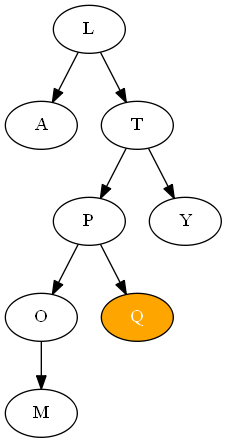
\includegraphics[width=5cm,height=5cm,keepaspectratio]{bin_boom_2}
		\caption{De knoop Q is het rechterkind van knoop P.}
		\label{fig:bin_boom_2}
	\end{figure}

	
		\item \textbf{Verwijderen} van een knoop onderscheidt drie gevallen: 
			\begin{enumerate}
				\item \textit{De knoop heeft geen kinderen}: dan kan de knoop eenvoudig verwijderd worden. Indien knoop Q verwijderdt wordt krijgen we terug de originele boom.
				
				\item \textit{De knoop heeft één kind}: In dit geval moet de ouder die naar de te verwijderen knoop wijst, nu wijzen naar het enige kind van de te verwijderen knoop. Indien we knoop P verwijderen, moet het linkerkind van knoop T nu wijzen naar knoop O. Op figuur \ref{fig:bin_boom_3} wordt dit gedemonstreerd.
				
				\begin{figure}[h]
					\centering
					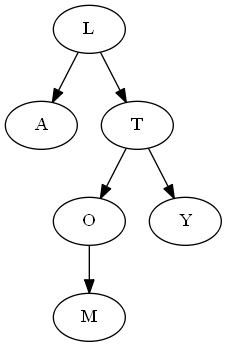
\includegraphics[width=5cm,height=5cm,keepaspectratio]{bin_boom_3}
					\caption{Verwijderen van de knoop P die slechts één kind heeft.}
					\label{fig:bin_boom_3}
				\end{figure}

			
				\item \textit{De knoop heeft twee kinderen}: In dit geval worden twee kinderen ouderloos. De te verwijderen knoop bevat echter zijn opvolger in de deelboom waarvan zijn rechterkind wortel van is. De opvolger is namelijk het kleinste element in deze deelboom. In het geval dat we knoop T verwijderen zal Y de ouder worden van O aangezien dit het kleinste (en ook enigste) element is in de deelboom, zoals op figuur \ref{fig:bin_boom_4} weergegeven.
				
				\begin{figure}[h]
					\centering
					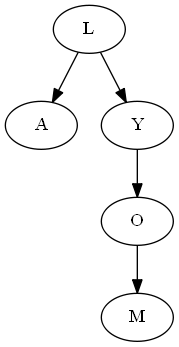
\includegraphics[width=5cm,height=5cm,keepaspectratio]{bin_boom_4}
					\caption{Verwijderen van de knoop T die twee kinderen heeft.}
					\label{fig:bin_boom_4}
				\end{figure}		
			\end{enumerate}
	\end{itemize}

	Een binaire boom is niet altijd efficiënt. Indien de sleutels ingelezen worden in volgorde, zal de binaire boom een gelinkte lijst voorstellen, waardoor de operaties $O(n)$ worden i.p.v. $O(\lg n)$.
	Dit probleem werd opgelost door bomen die zichzelf zo evenwichtig mogelijk trachten te houden. Er zijn drie soorten van deze bomen:
	\begin{enumerate}
		\item \textbf{Rood-zwarte bomen}. Dit soort bomen tracht elke operatie steeds efficiënt te maken door ervoor te zorgen dat de structuur van de boom nagenoeg perfect blijft. Dit is de meest robuste methode.
		\item \textbf{Splay trees}. Deze soort wordt de vorm van de boom meermaals aangepast, zodat de structuur van de boom nooit slecht is. Bij deze bomen is het gemiddelde geval steeds efficiënt (geamortiseerd), maar een individuele operatie kan soms slecht uitvallen.
		\item \textbf{Randomized search trees} (treap). Deze boomstructuur zorgt ervoor dat de boom zo willekeurig mogelijk blijft, ongeacht de volgorde van toevoegen of verwijderen. Dit zorgt ervoor dat de verwachtingswaarde van elke operatie $O(\lg n)$ is.
	\end{enumerate}
	\section{Rood-zwarte bomen}
	Gegeven Figuur \ref{fig:bin_boom_compleet}, een complete binaire boom. Indien we telkens elementen zouden verwijderen uit de linkerdeelboom van de wortel, zal deze binaire boom niet meer in evenwicht zijn zoals te zien op figuur \ref{fig:bin_boom_onevenwichtig}.
	
	\begin{figure}[h]
		\centering
		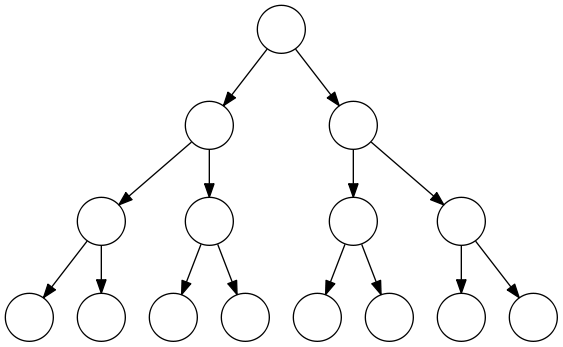
\includegraphics[width=8cm,height=8cm,keepaspectratio]{bin_boom_compleet}
		\caption{Een complete binaire boom.}
		\label{fig:bin_boom_compleet}
	\end{figure}

	\begin{figure}[h]
		\centering
		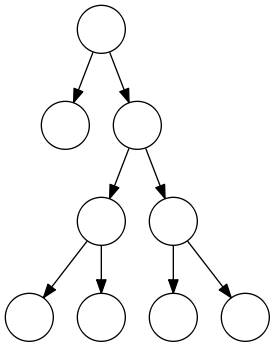
\includegraphics[width=5cm,height=5cm,keepaspectratio]{bin_boom_onevenwichtig}
		\caption{Een onevenwichtige binaire boom.}
		\label{fig:bin_boom_onevenwichtig}
	\end{figure}

	Een verbetering hierop is een 2-3-4 boom. Dit is een boom waarbij een knoop twee, drie of vier kinderen kan hebben waarbij alle bladeren even diep zitten. Een knoop kan één, twee of drie data-elementen bijhouden. Een voorbeeld van een dergelijke boom is te zien op figuur \ref{fig:2-3-4_boom}. De toevoeg operatie van de set \{48, 49, 50\} gebeurd als volgt: eerst wordt 48 toegevoegd aan het tweede data-element van de uiterst rechtse knoop. Het getal 49 kan geplaatst worden op het derde data-element. Op het moment dat 50 toegevoegd moet worden, kan er hiervoor geen nieuw kind aangemaakt worden aangezien alle bladeren op dezelfde diepte moet zitten. Daarom wordt de middelste knoop (48) naar de ouderknoop geplaatst, 49 op het tweede data-element en dan kan 50 uiteindelijk op het derde data-element komen. Figuur \ref{fig:2-3-4_boom_toegevoegd} toont de nieuwe 2-3-4 boom.
	
	\begin{figure}[h]
		\centering
		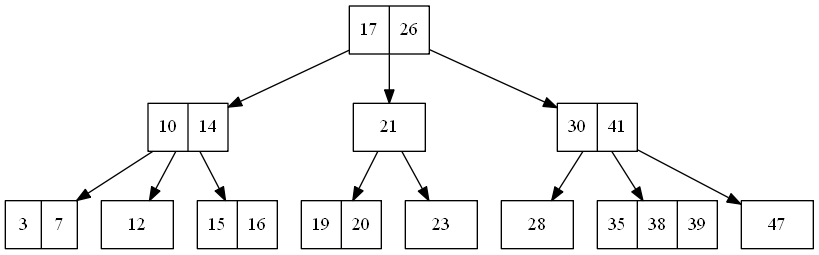
\includegraphics[width=11cm,height=11cm,keepaspectratio]{2-3-4_boom}
		\caption{Een 2-3-4 boom.}
		\label{fig:2-3-4_boom}
	\end{figure}

	\begin{figure}[h]
		\centering
		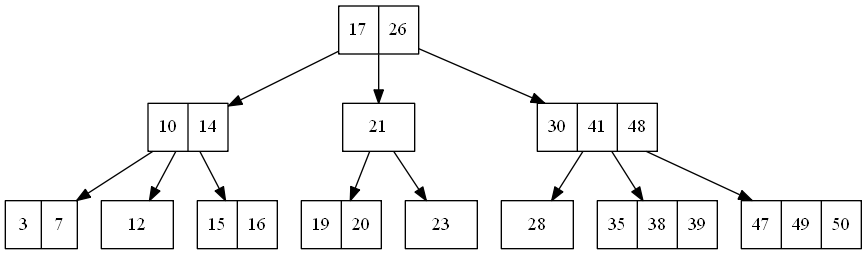
\includegraphics[width=11cm,height=11cm,keepaspectratio]{2-3-4_boom_toegevoegd}
		\caption{Een 2-3-4 boom waaraan de elementen 48, 49 en 50 zijn toegevoegd.}
		\label{fig:2-3-4_boom_toegevoegd}
	\end{figure}

	Een rood-zwarte boom simuleert een 2-3-4 boom. Figuur \ref{fig:2-3-4_to_rb} toont de conversie van 2 knopen van de 2-3-4 boom op figuur \ref{fig:2-3-4_boom}.
	\begin{figure}[h]
		\centering
		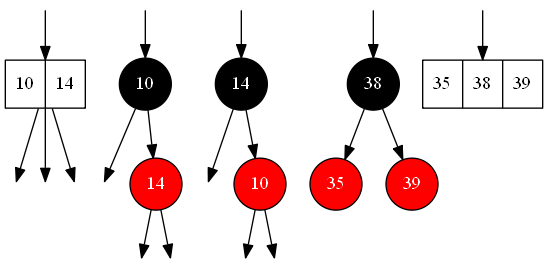
\includegraphics[width=10cm,height=10cm,keepaspectratio]{2-3-4_to_rb}
		\caption{Conversie 2-3-4 knopen naar rood-zwarte knopen.}
		\label{fig:2-3-4_to_rb}
	\end{figure}
	
	\subsection{Definitie rood-zwarte boom}
	Formeel kan een rood-zwarte zoekboom als volg gedefinieerd worden:
	\begin{itemize}
		\item Het is een binaire zoekboom.
		\item De knopen zijn rood of zwart (deze extra informatie kan bijgehouden worden met slechts één bit, aangezien er slechts twee kleuren zijn).
		\item Een rode knoop heeft \textit{nooit} een rood kind.
		\item Elke virtuele knoop is zwart. Een virtuele knoop is een kind van een blad-element waarbij de virtuele knoop geen gegevens bevat.
		\item De zwarte hoogte $z$ van een knoop $k$ is hetzelfde voor elk pad naar een virtuele knoop startend vanaf $k$, met $k$ niet meegerekend. De zwarte hoogte is het aantal zwarte knopen op dit pad.
	\end{itemize}
	Door deze voorwaarden is het gegarandeerd dat de kleinste deelboom minstens half zo diep is als de grootste deelboom. Bekijk figuur \ref{fig:rood-zwarte_boom}, waarop een geldige rood-zwarte boom te zien is. De zwarte hoogte van de wortel is 2, want voor elk pad naar een virtuele knoop is het aantal zwarte knopen 2. Een deelboom met wortel $w$ en zwarte hoogte $z$ zal minstens $2^z - 1$ inwendige knopen bevatten.
	\begin{figure}[h]
		\centering
		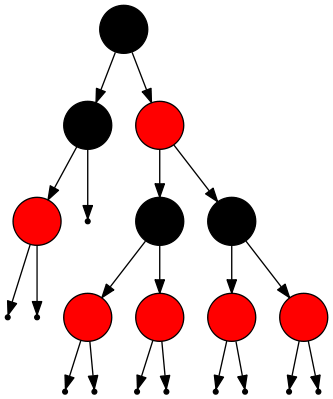
\includegraphics[width=4cm,height=4cm,keepaspectratio]{rood-zwarte_boom}
		\caption{Een rood-zwarte boom.}
		\label{fig:rood-zwarte_boom}
	\end{figure}
	
	\subsection{Rotaties}
	Bij het toevoegen of verwijderen van een element kan een rood-zwarte boom niet meer aan de voorwaarden voldoen. Rotaties zal de vorm van de boom aanpassen, maar zal de inorder volgorde behouden. Een rotatie is O(1).
   	\begin{figure}[h]
	   	\centering
	   	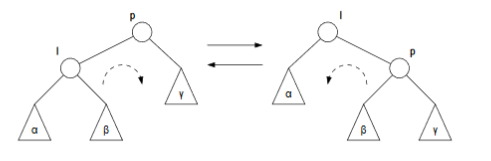
\includegraphics[width=0.75\textwidth]{rotaties}
	   	\caption{Rotaties.}
	   	\label{fig:rotaties}
    \end{figure}
	
	\subsection{Bottom-up rood-zwarte bomen}
	\begin{itemize}
		\item \textbf{Toevoegen.} Stel dat we een nieuwe knoop \textit{c} willen toevoegen. Een nieuwe knoop krijgt altijd een rode kleur want de zwarte diepte herstellen is een ingewikkelder proces. Indien de ouderknoop \textit{p} van \textit{c} een zwarte kleur heeft, is er geen probleem. Is de kleur van \textit{p} rood, dan zijn er zes gevallen mgoelijk, waarvan 3 het spiegelbeeld zijn van elkaar (afhankelijk of dat \textit{c} het linkerkind of rechterkind is van \textit{p}.
		\begin{enumerate}
			\item \textit{De broer b van p is rood}. 
		   	\begin{figure}[h]
				\centering
				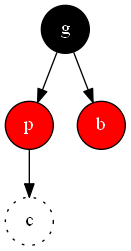
\includegraphics[width=5cm,height=5cm,keepaspectratio]{rode_broer}
				\caption{Rode broer.}
				\label{fig:rode_broer}
			\end{figure}
			In dit geval kan \textit{g} rood gemaakt worden. De knopen \textit{p} en \textit{b} kunnen op hun beurt dan zwart gemaakt worden. Indien \textit{g} een zwarte ouder heeft is de toevoegoperatie gelukt. Is de kleur van de ouder van \textit{g} rood, dan wordt het probleem opgeschoven waarbij \textit{g} nu de rol neemt van \textit{c}.
			\item \textit{De broer b van p is zwart}. In dit geval wordt er nog een onderscheidt gemaakt tussen de positie van \textit{c}.
			\begin{enumerate}
				\item \textit{Knoop c is een linkerkind van p}. Roteer \textit{p} en \textit{g} naar rechts, maak \textit{p} zwart en \textit{g} rood. Het probleem is opgelost.
				\item \textit{Knoop c is een rechterkind van p} Roteer \textit{p} en \textit{c} naar links, zodat vorige situatie bekomen wordt.
				
			\end{enumerate}
		\end{enumerate}
		\item \textbf{Verwijderen.}
	\end{itemize}
	
	\subsection{Top-down rood-zwarte bomen}
	
	


	
	\section{Splay trees}
	Splay trees zullen ervoor zorgen dat een reeks van operaties efficiënt is. Het kan dus voorkomen dat een individuele operatie traag uitvalt, maar dat de geamortiseerde performantie goed is. Een splay tree is eigenlijk een normale binaire boom waarbij één extra functie wordt toegevoegd, de splay-functie. Indien een knoop gezocht en gevonden wordt, zal de splay-functie ervoor zorgen dat deze knoop de wortel wordt van de boom. Dit kan een boom die de vorm van een gelinkte lijst heeft stelselmatig ombouwen tot een goede binaire boom. Een naïeve methode is echter om telkens de knoop te roteren met zijn ouder. Figuur \ref{fig:splay_tree_naief} toont het resultaat van deze operatie. In de linkse boom wordt de knoop F gezocht. Na het zoeken wordt de splay operatie uitgevoerd die altijd de knoop F zal roteren met zijn ouder. Het eindresultaat is terug een gelinkte lijst.
	\begin{figure}[h]
		\centering
		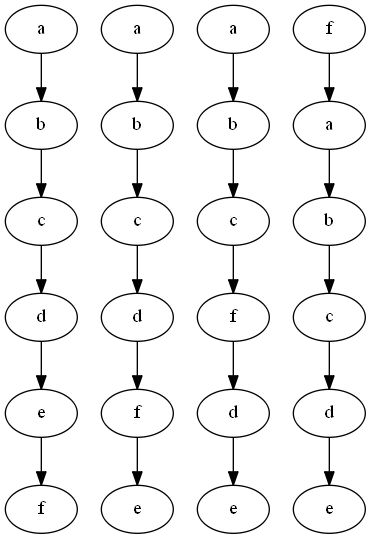
\includegraphics[width=5cm,height=5cm,keepaspectratio]{splay_tree_naief}
		\caption{Naïeve splay-functie.}
		\label{fig:splay_tree_naief}
	\end{figure}
	Een beter methode zou zijn om eerste E met D te roteren, dan F met E. De volgende stap roteert C met B, gevolgd door de rotatie F met C.
	\begin{figure}[h]
		\centering
		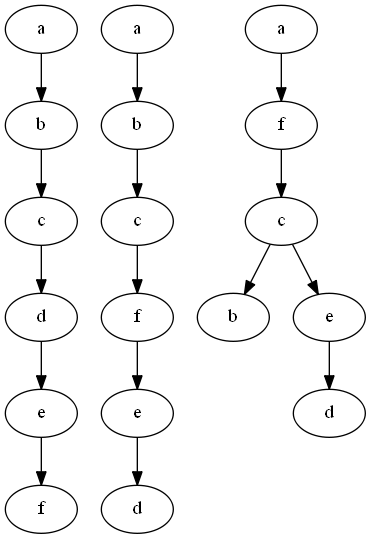
\includegraphics[width=7cm,height=7cm,keepaspectratio]{splay_tree_beter}
		\caption{Goede splay functie.}
		\label{fig:splay_tree_beter}
	\end{figure}

	\subsection{Performantie van splay trees}
	Omdat de vorm van de boom voortdurend verandert, wordt in het bewijs gebruik gemaakt van een potentiaalfunctie $\Phi$. Elke vorm van de boom krijgt een getal dat het potentiaal voorstelt. Een goede operatie zal het potentiaal verhogen terwijl een slechte operatie deze zal laten dalen. Stel $a_i$ de geamortiseerde tijd van een operatie, $t_i$ de werkelijke tijd van de operatie, $\Phi_i$ het potentiaal na de operatie en $\Phi_{i - 1}$ het potentiaal voor de operatie. $a_i$ kan beschreven worden als: 
	$$a_i = t_i + \Phi_i - \Phi_{i - 1}$$ Een reeks van operaties is de som van alle $a_i$:
	\begin{equation*}
	\begin{split}
		\sum_{i = 1}^{m} a_i & = \sum_{i = 1}^{m} (t_i + \Phi_i - \Phi_{i - 1}) \\
							   & =  \sum_{i = 1}^{m} (t_i + \Phi_m - \Phi_0)
	\end{split}
	\end{equation*}
	Hierbij is $\Phi_0$ de beginpotentiaal. De potentiaalfunctie moet zo gekozen worden zodat het eindpotentiaal niet kleiner is als het beginpotentiaal. Doorgaans wordt de potentiaalfunctie 
	$$\Phi = \sum_{i = 1}^m \lg s_i$$
	genomen. Hier is $s_i$ het aantal knopen in de deelboom waar knoop $i$ wortel van is. $\lg s_i$ wordt dan de rang van knoop $i$ genoemd.
	

	
	
	
\end{document}
